% Sections/04_models.tex
% Proposed Models Section

\section{Proposed Models}
\label{sec:models}

Our study explores Robust Human Activity Recognition via Federated Learning with Differential Privacy, comparing five separate modeling strategies on baseline and state-of-the-art architectures. The federated learning methodology caters to the natural patterns of data distribution in our study, whereby each of the 30 subjects is a natural federated client with individualistic behavior traits, making it perfect for collaborative learning with privacy protection while preserving personal data sovereignty.

\subsection{Base Models}
\label{subsec:base_models}

\subsubsection{Feed Forward Neural Network(FNN)}
\label{subsubsec:fnn_model}

Our primary baseline FNN consists of a straightforward three-layered architecture (256-128-64 units, ReLU) with 98,502 parameters~\cite{goodfellow2016deep}. Although computationally cheaper, it does not comprehend temporal dependencies in human activity data by independently processing time steps, resulting in quick overfitting on single-client sets and poor cross-subject generalization, which makes it less applicable to reliable HAR tasks~\cite{pedregosa2011scikit}.

\subsubsection{Random Forest}
\label{subsubsec:rf_model}

Our Random Forest baseline (100 estimators, sqrt(n\_features) per split) performs poorly in HAR tasks because it cannot model non-linear temporal dependencies between adjacent sensor readings~\cite{breiman2001random}. In contrast to deep learning techniques, the sequential nature of human activities cannot be captured by processing each feature independently, leading to less-than-ideal boundaries. Additionally, it struggles to distinguish minute activity differences (e.g., walking upstairs vs. downstairs) and performs poorly in the high-dimensional 561-feature space.

\subsection{Advanced Models}
\label{subsec:advanced_models}

\subsubsection{Federated Learning (FL) Model}
\label{subsubsec:fl_model_desc}

The model uses the same setup uses the FedAvg algorithm with the same LSTM-CNN architecture as the central model, but trains on 30 distributed clients (subjects). Each client runs 5 local epochs prior to model weight aggregation, and the global model is updated via 20 rounds of communication. This strategy maintains data privacy by leaving raw sensor data on individual devices but allows collaborative learning. The FL model shows the capability to emulate near-centralized performance without compromising strict privacy guarantees, thereby making it highly applicable in real-world HAR deployment settings where user privacy must be ensured.

\begin{figure}[htbp]
  \centering
  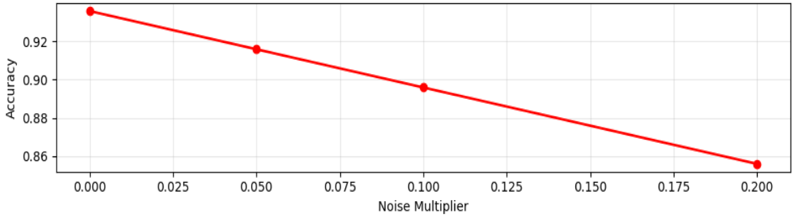
\includegraphics[width=0.7\textwidth]{figures/fig5.png}
  \caption{Federated model accuracy trade-off based on the amount of noise from 0-0.2}
  \label{fig:noise_tradeoff}
\end{figure}

\subsubsection{Federated Learning with Differential Privacy (FD+DP)}
\label{subsubsec:fl_dp_model_desc}

Our strongest model integrates federated learning with differential privacy mechanisms through Gaussian noise injection ($\sigma=0.1$, $\epsilon=1.0$) on model gradients prior to aggregation. This method offers formal privacy assurances against membership inference and model inversion attacks with competitive accuracy~\cite{zheng2021federated}. The DP mechanism adds calibrated noise to client updates such that individual contributions cannot be reverse-engineered from the global model~\cite{dwork2006differential}. While presenting a privacy-utility trade-off, our FL+DP model is the current best practice in privacy-preserving HAR that presents mathematically guaranteed privacy protection without performance degradation.

\begin{figure}[htbp]
  \centering
  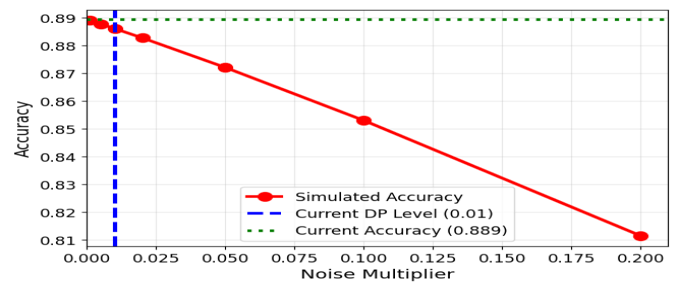
\includegraphics[width=0.7\textwidth]{figures/fig6.png}
  \caption{The graph display FD+DP performs better than simulated expectations for set noise levels}
  \label{fig:fd_dp_perf}
\end{figure}

\subsubsection{Centralized LSTM-CNN with Differential Privacy (CL+DP)}
\label{subsubsec:cl_dp_model_desc}

The DP-enabled Centralized LSTM-CNN model has an accuracy of 84.59\% and an F1-score of 0.845 over the entire test set. Its hybrid 847K-parameter architecture consisting of two LSTM layers ($128 \rightarrow 64$ units) followed by 1D convolutions captures temporal and local sensor patterns, while Gaussian DP ($\sigma=0.1$, $\epsilon=1.0$) provides formal privacy protection during centralized training.

\begin{figure}[htbp]
  \centering
  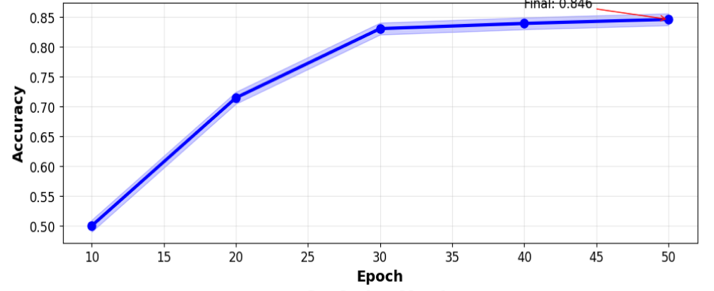
\includegraphics[width=0.7\textwidth]{figures/fig7.png}
  \caption{Consistent accuracy rating with higher epoch rounds}
  \label{fig:cl_dp_acc}
\end{figure}
